\documentclass[a4paper,10pt]{article}
\usepackage{epsfig}
\usepackage{latexsym}
\usepackage{graphicx}
\usepackage{amsfonts}
\usepackage{amsmath}
\usepackage{xcolor}

%-----------------------------------------
% Pour accepter les lettres accentuees de clavier azerty
% sans les \'e (utile) pour tapper directement en azerty 
% et ou faire passer aspell -c --lang=fr bidon.tex
%\usepackage[latin1]{inputenc}
%------------------------------------------


%\topmargin=-3cm
\topmargin=-1cm
\oddsidemargin=-1cm
\evensidemargin=-1cm
\textwidth=17cm
%\textheight=27cm
\textheight=25cm
\raggedbottom
\sloppy

\definecolor{Blue}{rgb}{0.,0.,1.}
\definecolor{LightSkyBlue}{rgb}{0.691,0.827,1.}
\definecolor{Red}{rgb}{1.,0.,0.}
\definecolor{Green}{rgb}{0.,1.,0.}
\definecolor{Purple}{rgb}{0.5, 0., 0.5}
\definecolor{Try}{rgb}{0.15,0.,1}
\definecolor{Black}{rgb}{0., 0., 0.}

%To get DRAFT accross all pages
%\usepackage{draftcopy}
%To replace ``DRAFT'' by ``ON GOING''
%\draftcopyName{ON GOING}{150}

\title{Scanning speed and sampling in polarized mode}
\author{N.~Ponthieu}

\begin{document}
\maketitle
\tableofcontents

\begin{abstract}
This notes collects a few equations that define the constraints on the scanning
speed and the HWP rotation frequency. We first address beammaps on bright
sources for which we need to scan as fast as possible to match acquisition
constraints (max. scan duration = 30\,mn). We then talk about the other extreme
case where we observe faint sources.
\end{abstract}

\section{Polarized beammaps}

Let's call $N$ the number of points per FWHM that define the Nyquist
criterion. This criterion is loosely defined for a Gaussian beam to between 2 to
3 points per FWHM depending on the authors, but has never been set to lower than
2. In practice, we've been doing beammaps in total power with $N=2.5$.\\

If the HWP rotates mechanically at $\nu_{HWP}$\,Hz, it modulates the polarization
at $4\times\nu_{HWP}$, so we can reconstruct a full set of $I,Q,U$ parameters
per quarter of HWP rotation and so, as far as periods are concerned, $T_{pol} =
T_{HWP}/4$. Let's call $T_{FWHM}$ the beam crossing time and put it
alltogether. The Nyquist criterion is satisfied if:

\begin{eqnarray}
T_{FWHM} &\geq& N\,T_{pol} \\
\frac{FWHM}{v} &\geq &N\frac{T_{HW}}{4}\\
v  &\leq & \frac{FWHM\times 4\,\nu_{HWP}}{N}
\end{eqnarray}

If we take $FWHM=11$\,arcsec and $N=2.5$, this leads to $v \leq
52.45$\,arcec/s.\\

Total power beammaps are scanned at 65\,arcsec/s for total scan duration of
about 25\,mn. Adjusting the speed would lead to approximate 31\,mn scans that
are larger than the maximum scan duration of the acquisition 30\,mn. However,
dropping the requirement to 2.2 points per FWHM and allowing for scanning speed
of 60\,arcsec/s should not degrade the beammap so much and would allow us to
match the scan duration limit.

\section{Faint sources}

In the case of a beammap with a bright source, we probably can be less stringent
on the removal of HWPSS. For observations of weak sources however, we should be
more careful about this. The FWHM couples to the scanning speed to produce a
lowpass on time series. If this lowpass is now low enough before the HWP
rotation frequency, than it is possible that residuals of the HWPSS at these
harmonics are mixed with the signal.

Figures~\ref{fig:bhss} illustrates this effect for 3 different scanning speeds
in the case of HWP rotated at 3Hz. Typically, to ensure a -3\,dB cutoff at 3Hz, we must
thus scan no faster than 23.5\,arcsec/s. In practice, we'll thus limit ourselves
to 25\,arcsec/s.

\begin{figure}
\begin{center}
\includegraphics[scale=1,angle=0]{Figures/beam_hwp_scanning_speed.eps}
\caption{Beam cutoff as a function of scanning speed (at 1mm,
  FWHM=11\,arcsec) vs HWP rotation frequencies.}
\label{fig:bhss}
\end{center}
\end{figure}


%----------------------------------------------------------------------------------------
\begin{thebibliography}{}
\end{thebibliography}

\end{document}
